\chapter{Réactions péricycliques}\label{ch:b3:pericyclic}

La lumière du soleil qui tombe sur la peau ouvre un cycle du
7-déhydrocholestérol en une fraction de seconde~; la chaleur du corps
déplace ensuite un atome d'hydrogène à travers sept atomes de carbone, et
le produit est la vitamine D$_3$. Aucune des deux étapes ne comporte
d'intermédiaire~: les liaisons se rompent et se forment ensemble, autour
d'un cycle d'atomes, en passant par un seul état de transition. La première
étape n'a lieu qu'à la lumière et la seconde qu'à la chaleur, et chacune
donne un seul stéréoisomère. Ce chapitre explique pourquoi, à partir de la
symétrie des orbitales moléculaires mises en jeu~: les règles trouvées par
Robert Woodward et Roald Hoffmann, qui prévoient si une telle réaction peut
avoir lieu et ce qu'elle donne.

\begin{recall}
Le volume de deuxième année a donné les coefficients de Hückel des
polyènes, les cycles aromatiques et antiaromatiques, la HOMO, la LUMO et
les orbitales frontières, les réactions concertées, et la réaction de
Diels--Alder d'un diène avec un diénophile avec sa règle endo~; le volume de
première année, les descripteurs \textit{Z}/\textit{E}. Le \cref{ch:b3:point-groups} a défini l'axe $C_2$
et le plan miroir, le \cref{ch:b3:photochemistry} les états excités et la
photocycloaddition [2+2].
\end{recall}

\begin{omfigure}
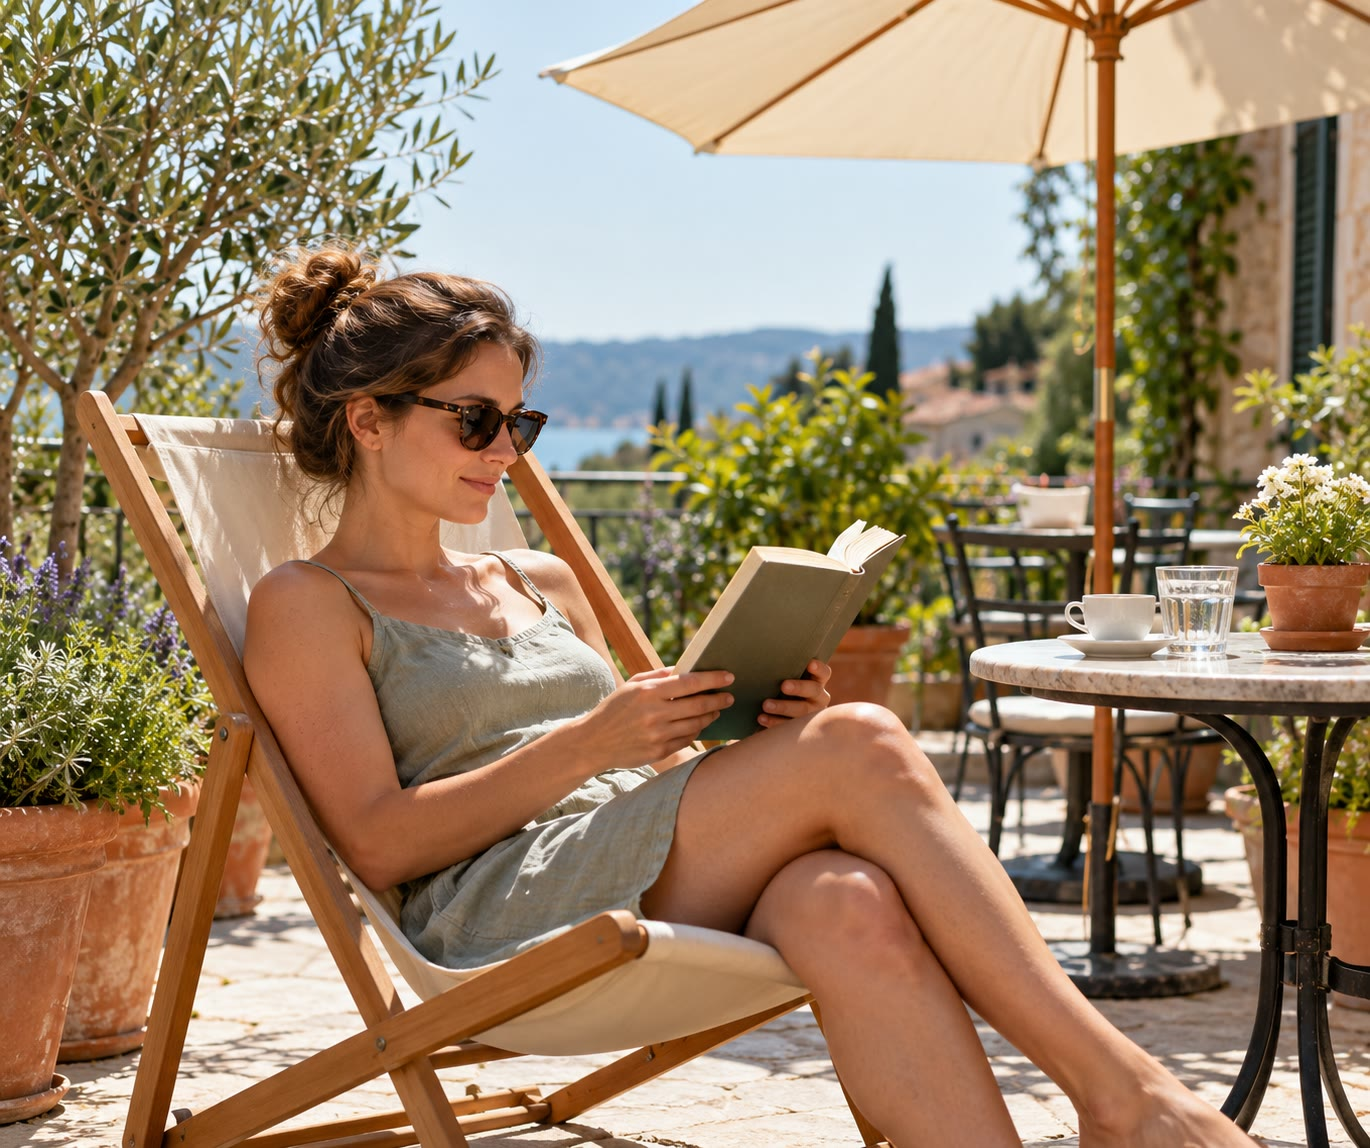
\includegraphics[width=0.55\linewidth]{images/book4/ai/b3-26-terrace.jpg}

{\small Lecture sur une terrasse ensoleillée~: la lumière ultraviolette qui
atteint la peau amorce la synthèse de la vitamine D$_3$ par une ouverture de cycle péricyclique.}
\end{omfigure}

\section{Quatre familles}

\begin{definition}[Réaction péricyclique]\label{def:b3:pericyclic:pericyclic}
Une \emph{réaction péricyclique}\index{reaction pericyclique@réaction péricyclique} est une réaction concertée
dont l'état de transition est un arrangement cyclique d'orbitales en
interaction, dans lequel toutes les liaisons se forment et se rompent
autour du cycle en même temps.
\end{definition}

\begin{definition}[Familles de réactions péricycliques]\label{def:b3:pericyclic:families}
Dans une \emph{réaction électrocyclique}\index{reaction electrocyclique@réaction électrocyclique}, un polyène conjugué
se referme en cycle en formant une liaison $\sigma$ entre ses extrémités, ou
l'inverse. Dans une \emph{cycloaddition}\index{cycloaddition}, deux systèmes $\pi$ s'unissent
en un cycle en formant deux liaisons $\sigma$~; une cycloaddition $[m + n]$ réunit des composantes
de $m$ et $n$ atomes (ou électrons). Dans un \emph{réarrangement sigmatropique}\index{rearrangement sigmatropique@réarrangement sigmatropique}, une liaison $\sigma$ migre le long d'un système
$\pi$~; dans une migration $[i, j]$, la liaison passe des atomes 1 et 1 aux atomes $i$ et $j$
des deux fragments. Une \emph{réaction chélétropique}\index{reaction cheletropique@réaction chélétropique}
forme ou rompt deux liaisons sur un même atome, comme lorsque le dioxyde de
soufre quitte un sulfolène. Dans une \emph{réaction ène}\index{reaction ene@réaction ène}, un alcène
porteur d'un hydrogène allylique s'additionne sur une liaison $\pi$, l'hydrogène se déplaçant avec lui.
\end{definition}

\begin{definition}[Suprafacial et antarafacial]\label{def:b3:pericyclic:faciality}
Une composante réagit de façon \emph{suprafaciale}\index{suprafacial} lorsque ses deux
nouvelles liaisons se forment, ou ses deux anciennes se rompent, sur la même face de son système $\pi$ (ou avec
rétention sur une liaison $\sigma$), et de façon \emph{antarafaciale}\index{antarafacial}
lorsqu'elles sont sur des faces opposées (ou avec inversion).
\end{definition}

\section{Réactions électrocycliques}

\begin{definition}[Conrotatoire et disrotatoire]\label{def:b3:pericyclic:rotation-modes}
Lors d'une fermeture de cycle électrocyclique, les deux groupes terminaux
tournent autour des liaisons qui les relient à la chaîne. La rotation est
\emph{conrotatoire}\index{conrotatoire} lorsqu'ils tournent tous deux dans
le même sens (tous deux dans le sens horaire, vus le long de la chaîne), et
\emph{disrotatoire}\index{disrotatoire} lorsqu'ils tournent en sens
opposés.
\end{definition}

\begin{theorem}[Réactions électrocycliques]\label{thm:b3:pericyclic:electrocyclic}
Une \omterm{def:b3:pericyclic:families}{réaction électrocyclique} thermique d'un polyène à $4n$ électrons $\pi$ est
\omterm{def:b3:pericyclic:rotation-modes}{conrotatoire}, et à $4n + 2$ électrons $\pi$ \omterm{def:b3:pericyclic:rotation-modes}{disrotatoire}.
\end{theorem}

\begin{proof}
La nouvelle liaison $\sigma$ se forme à partir des orbitales p terminales de la HOMO, qui
dans la réaction thermique contient les électrons de plus haute énergie~;
elle n'est liante que si les lobes qui se tournent l'un vers l'autre ont le
même signe. D'après la formule de Hückel
(\cref{ch:b3:solid-state}), les coefficients de l'orbitale $k$ d'une chaîne de $N$ atomes sont
proportionnels à $\sin(jk\pi/(N + 1))$, si bien que les deux extrémités, $j = 1$ et $j = N$, ont
pour coefficients $\sin(k\pi/(N + 1))$ et $\sin(Nk\pi/(N + 1)) = (-1)^{k+1}\sin(k\pi/(N + 1))$~: de même signe pour $k$ impair,
de signes opposés pour $k$ pair. Avec $N$ atomes et $N$ électrons, la HOMO est
$k = N/2$. Pour $N = 4n$, $k = 2n$ est pair~: les lobes supérieurs des extrémités ont des signes
opposés, et les deux extrémités doivent tourner dans le même sens, chacune
amenant vers l'intérieur son lobe du bon signe~: \omterm{def:b3:pericyclic:rotation-modes}{conrotatoire}. Pour $N = 4n + 2$, $k = 2n + 1$ est impair~: les lobes supérieurs
ont le même signe, et les tourner l'un vers l'autre est \omterm{def:b3:pericyclic:rotation-modes}{disrotatoire}.
\end{proof}

\begin{omfigure}
\begin{tikzpicture}[font=\small, >=Stealth]
  % butadiene HOMO psi2: 0.60 0.37 -0.37 -0.60 (lobes scaled x1.6)
  \foreach \x/\c in {0/0.60, 1/0.37, 2/-0.37, 3/-0.60} {
    \pic at (\x,0) {omp={1.6*\c}{90}};
    \fill (\x,0) circle (1.2pt);
  }
  \draw[black!60] (0,0) -- (3,0);
  \draw[->, thick, omThm] (-0.45,0.55) arc[start angle=130, end angle=20, radius=0.7];
  \draw[->, thick, omThm] (2.55,0.55) arc[start angle=130, end angle=20, radius=0.7];
  \node[font=\scriptsize, align=center] at (1.5,-1.3) {butadiène, $\psi_2$ (HOMO, 4 électrons)~:\\ extrémités de signes opposés~: \textbf{conrotatoire}};
  \begin{scope}[xshift=6.2cm]
  % hexatriene HOMO psi3: 0.52 0.23 -0.42 -0.42 0.23 0.52
  \foreach \x/\c in {0/0.52, 0.8/0.23, 1.6/-0.42, 2.4/-0.42, 3.2/0.23, 4.0/0.52} {
    \pic at (\x,0) {omp={1.6*\c}{90}};
    \fill (\x,0) circle (1.2pt);
  }
  \draw[black!60] (0,0) -- (4.0,0);
  \draw[->, thick, omThm] (-0.45,0.55) arc[start angle=130, end angle=20, radius=0.7];
  \draw[->, thick, omThm] (4.45,0.55) arc[start angle=50, end angle=160, radius=0.7];
  \node[font=\scriptsize, align=center] at (2.0,-1.3) {hexatriène, $\psi_3$ (HOMO, 6 électrons)~:\\ extrémités de même signe~: \textbf{disrotatoire}};
  \end{scope}
\end{tikzpicture}

{\small La HOMO du butadiène et de l'hexatriène, avec des lobes
proportionnels à leurs coefficients de Hückel (en bleu et en orange~: les
deux signes), dessinée le long de la chaîne. Pour qu'une liaison se forme
entre les extrémités, les lobes qui se tournent l'un vers l'autre doivent
avoir le même signe~: les deux extrémités tournent dans le sens horaire
dans le butadiène, en sens opposés dans l'hexatriène (flèches rouges).}
\end{omfigure}

La règle est stéréospécifique. Le (\textit{E},\textit{E})-hexa-2,4-diène, chauffé, se
fermerait de façon \omterm{def:b3:pericyclic:rotation-modes}{conrotatoire} en \textit{trans}-3,4-diméthylcyclobutène~; en pratique, c'est le cyclobutène
tendu qui s'ouvre, et le \textit{cis}-3,4-diméthylcyclobutène s'ouvre
de façon \omterm{def:b3:pericyclic:rotation-modes}{conrotatoire} en (\textit{E},\textit{Z})-hexa-2,4-diène uniquement. Le (\textit{E},\textit{Z},\textit{E})-octa-2,4,6-triène se ferme
de façon \omterm{def:b3:pericyclic:rotation-modes}{disrotatoire} en \textit{cis}-5,6-diméthylcyclohexa-1,3-diène.

\begin{proposition}[Réactions électrocycliques photochimiques]\label{prop:b3:pericyclic:photo-electrocyclic}
Sous irradiation, les règles s'inversent~: $4n$ électrons, \omterm{def:b3:pericyclic:rotation-modes}{disrotatoire}~; $4n + 2$, \omterm{def:b3:pericyclic:rotation-modes}{conrotatoire}.
\end{proposition}

\begin{proof}
L'absorption d'un photon fait passer un électron de la HOMO $k = N/2$ à la LUMO $k = N/2 + 1$
(\cref{ch:b3:photochemistry}), qui devient l'orbitale occupée la plus haute
et contrôle les extrémités. Son $k$ a la parité opposée, si bien que le signe relatif de ses
coefficients terminaux est inversé, et avec lui le sens de rotation.
\end{proof}

\begin{method}[Prévoir la stéréochimie d'une réaction électrocyclique]\label{met:b3:pericyclic:predict-stereo}
\begin{enumerate}
  \item Compter les électrons $\pi$ du polyène à chaîne ouverte ($4n$ ou $4n + 2$)~; noter s'il y a
        chauffage ou irradiation.
  \item Lire le mode~: thermique, $4n$ con, $4n + 2$ dis~; photochimique, l'inverse.
  \item Dessiner les extrémités avec leurs substituants, dans la
        conformation qui se ferme (s-cis)~; les tourner de 90° selon le mode
        choisi.
  \item Lire si les deux substituants aboutissent sur la même face du cycle
        (\textit{cis}) ou sur des faces opposées (\textit{trans}). Pour une ouverture de cycle, mener la même
        analyse à rebours.
\end{enumerate}
\end{method}

\section{Diagrammes de corrélation orbitalaire}

L'argument original de Woodward et Hoffmann considère toutes les
orbitales, pas seulement la HOMO. Le long d'un chemin \omterm{def:b3:pericyclic:rotation-modes}{conrotatoire}, la
molécule conserve un axe $C_2$~; le long d'un chemin
\omterm{def:b3:pericyclic:rotation-modes}{disrotatoire}, un plan miroir $\sigma$. Chaque orbitale du réactif et du
produit est symétrique (S) ou antisymétrique (A) par rapport à l'élément
conservé.

\begin{definition}[Diagramme de corrélation orbitalaire]\label{def:b3:pericyclic:orbital-correlation}
Un \emph{diagramme de corrélation orbitalaire}\index{diagramme de correlation orbitalaire@diagramme de corrélation orbitalaire} relie
chaque orbitale du réactif à l'orbitale du produit de même symétrie, par
rapport aux \omterm{def:b3:point-groups:operation}{éléments de symétrie} conservés le long du chemin réactionnel,
en les prenant dans l'ordre des énergies~: la S la plus basse avec la S la
plus basse, et ainsi de suite.
\end{definition}

\begin{proposition}[Conservation de la symétrie des orbitales]\label{prop:b3:pericyclic:correlation}
Si chaque orbitale occupée du réactif est corrélée à une orbitale occupée
du produit, la réaction thermique est permise~; si une orbitale occupée est
corrélée à une orbitale vide, elle est interdite, avec une barrière élevée.
\end{proposition}

\begin{proof}[Justification]
Le long du chemin, une orbitale garde sa symétrie et son énergie varie
continûment~; des orbitales de même symétrie ne peuvent pas se croiser
(elles se mélangent et se repoussent), celles de symétries différentes le
peuvent. Lorsqu'une orbitale doublement occupée du réactif doit devenir une
orbitale antiliante du produit, l'état fondamental du réactif conduit à un
état doublement excité du produit, et l'énergie de l'état fondamental
monte fortement jusqu'à ce que, tard sur le chemin, les états de même
symétrie se mélangent~: la barrière est élevée.
\end{proof}

\begin{omfigure}
\begin{tikzpicture}[font=\scriptsize]
  \foreach \px/\title/\el in {0/disrotatoire~: $\sigma$ conservé/s, 7.6/conrotatoire~: $C_2$ conservé/c} {
    \begin{scope}[xshift=\px cm]
    \node[font=\small\bfseries] at (2.0,5.1) {\title};
    \node at (0,4.7) {butadiène};
    \node at (4.0,4.7) {cyclobutène};
    \end{scope}
  }
  % ---- disrotatory (mirror): butadiene psi1 S, psi2 A, psi3 S, psi4 A;
  %      cyclobutene sigma S, pi S, pi* A, sigma* A
  \pic (b1) at (0,0.6) {omlevel={ud}{1.0}}; \node[anchor=east] at (-0.6,0.6) {$\psi_1$ S};
  \pic (b2) at (0,1.8) {omlevel={ud}{1.0}}; \node[anchor=east] at (-0.6,1.8) {$\psi_2$ A};
  \pic (b3) at (0,3.0) {omlevel={}{1.0}}; \node[anchor=east] at (-0.6,3.0) {$\psi_3$ S};
  \pic (b4) at (0,4.1) {omlevel={}{1.0}}; \node[anchor=east] at (-0.6,4.1) {$\psi_4$ A};
  \pic (c1) at (4.0,0.1) {omlevel={ud}{1.0}}; \node[anchor=west] at (4.6,0.1) {$\sigma$ S};
  \pic (c2) at (4.0,1.3) {omlevel={ud}{1.0}}; \node[anchor=west] at (4.6,1.3) {$\pi$ S};
  \pic (c3) at (4.0,3.4) {omlevel={}{1.0}}; \node[anchor=west] at (4.6,3.4) {$\pi^*$ A};
  \pic (c4) at (4.0,4.4) {omlevel={}{1.0}}; \node[anchor=west] at (4.6,4.4) {$\sigma^*$ A};
  \draw[omcorr] (b1-r) -- (c1-l);
  \draw[omcorrforbidden] (b2-r) -- (c3-l);
  \draw[omcorr] (b3-r) -- (c2-l);
  \draw[omcorr] (b4-r) -- (c4-l);
  % ---- conrotatory (C2): butadiene psi1 A, psi2 S, psi3 A, psi4 S;
  %      cyclobutene sigma S, pi A, pi* S, sigma* A
  \begin{scope}[xshift=7.6cm]
  \pic (d1) at (0,0.6) {omlevel={ud}{1.0}}; \node[anchor=east] at (-0.6,0.6) {$\psi_1$ A};
  \pic (d2) at (0,1.8) {omlevel={ud}{1.0}}; \node[anchor=east] at (-0.6,1.8) {$\psi_2$ S};
  \pic (d3) at (0,3.0) {omlevel={}{1.0}}; \node[anchor=east] at (-0.6,3.0) {$\psi_3$ A};
  \pic (d4) at (0,4.1) {omlevel={}{1.0}}; \node[anchor=east] at (-0.6,4.1) {$\psi_4$ S};
  \pic (e1) at (4.0,0.1) {omlevel={ud}{1.0}}; \node[anchor=west] at (4.6,0.1) {$\sigma$ S};
  \pic (e2) at (4.0,1.3) {omlevel={ud}{1.0}}; \node[anchor=west] at (4.6,1.3) {$\pi$ A};
  \pic (e3) at (4.0,3.4) {omlevel={}{1.0}}; \node[anchor=west] at (4.6,3.4) {$\pi^*$ S};
  \pic (e4) at (4.0,4.4) {omlevel={}{1.0}}; \node[anchor=west] at (4.6,4.4) {$\sigma^*$ A};
  \draw[omcorr] (d1-r) -- (e2-l);
  \draw[omcorr] (d2-r) -- (e1-l);
  \draw[omcorr] (d3-r) -- (e4-l);
  \draw[omcorr] (d4-r) -- (e3-l);
  \end{scope}
\end{tikzpicture}

{\small \omterm{def:b3:pericyclic:orbital-correlation}{Diagrammes de corrélation orbitalaire} pour butadiène $\rightleftharpoons$ cyclobutène. À gauche, le
chemin \omterm{def:b3:pericyclic:rotation-modes}{disrotatoire} conserve un plan miroir~: la $\psi_2$ occupée (A) est corrélée à la
$\pi^*$ vide (A) du cyclobutène (tirets rouges)~: thermiquement interdit. À
droite, le chemin \omterm{def:b3:pericyclic:rotation-modes}{conrotatoire} conserve un axe $C_2$~: les orbitales
occupées vont vers des orbitales occupées~: thermiquement permis.}
\end{omfigure}

\begin{method}[Construire un diagramme de corrélation]\label{met:b3:pericyclic:correlation-diagram}
\begin{enumerate}
  \item Trouver les \omterm{def:b3:point-groups:operation}{éléments de symétrie} qui coupent en deux les liaisons
        formées et rompues et qui sont conservés tout au long du chemin
        choisi.
  \item Lister les orbitales qui participent, du réactif et du produit,
        dans l'ordre des énergies, et étiqueter chacune S ou A pour chaque
        élément.
  \item Relier l'orbitale la plus basse de chaque type de symétrie d'un
        côté à la plus basse du même type de l'autre côté, puis la suivante,
        sans jamais croiser deux lignes de même symétrie.
  \item Examiner les orbitales occupées~: toutes vers des occupées,
        permis~; une vers une vide, interdit.
\end{enumerate}
\end{method}

\begin{definition}[Diagramme de corrélation des états]\label{def:b3:pericyclic:state-correlation}
Un \emph{diagramme de corrélation des états}\index{diagramme de correlation des etats@diagramme de corrélation des états} relie les
états électroniques du réactif et du produit, construits chacun à partir
des configurations orbitalaires et étiquetés par leur symétrie globale, le
long du chemin~; des états de même symétrie ne se croisent pas.
\end{definition}

Pour le chemin \omterm{def:b3:pericyclic:rotation-modes}{disrotatoire} interdit, l'état fondamental du butadiène ($\psi_1^2\psi_2^2$)
est corrélé à un état doublement excité du cyclobutène ($\sigma^2\pi^{*2}$), mais le premier état
excité ($\psi_1^2\psi_2\psi_3$) est corrélé au premier état excité du cyclobutène ($\sigma^2\pi\pi^*$)~: à partir de
l'état excité, le chemin \omterm{def:b3:pericyclic:rotation-modes}{disrotatoire} est descendant. C'est l'inversion
photochimique de la \cref{prop:b3:pericyclic:photo-electrocyclic}, vue sur
les états.

\section{Cycloadditions}

\begin{theorem}[Cycloadditions]\label{thm:b3:pericyclic:cycloaddition}
Une \omterm{def:b3:pericyclic:families}{cycloaddition} $[m + n]$ thermique dans laquelle les deux composantes réagissent de façon
\omterm{def:b3:pericyclic:faciality}{suprafaciale} est permise lorsque $m + n = 4q + 2$ électrons, et interdite lorsque $m + n = 4q$~; sous irradiation, la
règle s'inverse.
\end{theorem}

\begin{proof}
Les deux nouvelles liaisons se forment entre la HOMO d'une composante et la
LUMO de l'autre, qui se font face par leurs lobes terminaux~; les deux
réagissant de façon \omterm{def:b3:pericyclic:faciality}{suprafaciale}, les deux liaisons ne sont liantes que si
les coefficients terminaux de la HOMO et de la LUMO ont le même signe
relatif. Pour une composante de $N$
électrons sur $N$ atomes, la HOMO a $k = N/2$ et la LUMO $k = N/2 + 1$~; coefficients terminaux de
même signe pour $k$ impair, opposés pour $k$ pair. Dans le cas [4+2], la HOMO du diène ($k = 2$)
et la LUMO de l'éthène ($k = 2$) ont toutes deux des signes terminaux opposés~: elles s'accordent. Dans le
cas [2+2], la HOMO d'un éthène ($k = 1$, mêmes signes) rencontre la LUMO de l'autre
($k = 2$, signes opposés)~: une extrémité liante, une antiliante. En général, la HOMO de la composante $m$
et la LUMO de la composante $n$ s'accordent lorsque $m/2$ et $n/2 + 1$ ont la même
parité, c'est-à-dire lorsque $(m + n)/2$ est impair~: $m + n = 4q + 2$. Sous irradiation, la LUMO
simplement occupée de la composante excitée joue le rôle de sa HOMO, et la
condition de parité s'inverse.
\end{proof}

\begin{omfigure}
\begin{tikzpicture}[font=\scriptsize]
  % [4+2]: diene HOMO above, ethene LUMO (pi*) below, facing lobes match at both ends
  \foreach \x/\c in {0/0.60, 1/0.37, 2/-0.37, 3/-0.60} {
    \pic at (\x,1.6) {omp={1.4*\c}{90}}; \fill (\x,1.6) circle (1.1pt);
  }
  \draw[black!60] (0,1.6) -- (3,1.6);
  \foreach \x/\c in {0/-0.71, 3/0.71} {
    \pic at (\x,-0.4) {omp={1.4*\c}{90}}; \fill (\x,-0.4) circle (1.1pt);
  }
  \draw[black!60] (0,-0.4) -- (3,-0.4);
  \draw[omMeth, densely dashed, thick] (-0.25,0.75) -- (-0.25,0.35) (3.25,0.75) -- (3.25,0.35);
  \node[omMeth] at (-0.25,0.55) [left] {liante};
  \node[omMeth] at (3.25,0.55) [right] {liante};
  \node[font=\small] at (1.5,2.95) {[4+2]~: HOMO du diène};
  \node[font=\small] at (1.5,-1.75) {LUMO de l'éthène~: permise};
  \begin{scope}[xshift=7.2cm]
  \foreach \x/\c in {0/0.71, 3/0.71} {
    \pic at (\x,1.6) {omp={1.4*\c}{90}}; \fill (\x,1.6) circle (1.1pt);
  }
  \draw[black!60] (0,1.6) -- (3,1.6);
  \foreach \x/\c in {0/-0.71, 3/0.71} {
    \pic at (\x,-0.4) {omp={1.4*\c}{90}}; \fill (\x,-0.4) circle (1.1pt);
  }
  \draw[black!60] (0,-0.4) -- (3,-0.4);
  \draw[omMeth, densely dashed, thick] (-0.25,0.75) -- (-0.25,0.35);
  \draw[omThm, densely dashed, thick] (3.25,0.75) -- (3.25,0.35);
  \node[omMeth] at (-0.25,0.55) [left] {liante};
  \node[omThm] at (3.25,0.55) [right] {antiliante};
  \node[font=\small] at (1.5,2.95) {[2+2]~: HOMO de l'éthène};
  \node[font=\small] at (1.5,-1.75) {LUMO de l'éthène~: interdite};
  \end{scope}
\end{tikzpicture}

{\small Orbitales frontières face à face dans des \omterm{def:b3:pericyclic:families}{cycloadditions}
\omterm{def:b3:pericyclic:faciality}{suprafaciales} (les lobes inférieurs de la composante du haut rencontrent les
lobes supérieurs de celle du bas~; taille des lobes d'après les
coefficients de Hückel). Dans la réaction [4+2], les deux nouvelles
liaisons sont liantes~; dans la réaction [2+2], une extrémité est liante et
l'autre antiliante.}
\end{omfigure}

Thermiquement, deux alcènes ne donnent pas un cyclobutane en une seule
étape concertée~; sous irradiation, si (\cref{ch:b3:photochemistry}). Les
cétènes sont l'exception qui confirme la règle~: leur orbitale $\pi^*$ C=O, perpendiculaire à celle de C=C, leur permet de
réagir avec un alcène selon une géométrie [$\pi2_s$ + $\pi2_a$], une composante \omterm{def:b3:pericyclic:faciality}{suprafaciale} et le
cétène \omterm{def:b3:pericyclic:faciality}{antarafacial}, et ils forment des cyclobutanones par voie thermique.

\begin{definition}[Cycloadditions 1,3-dipolaires]\label{def:b3:pericyclic:dipolar}
Un \emph{dipôle 1,3}\index{dipole 1,3@dipôle 1,3} est un système $\pi$ de trois atomes à quatre
électrons, écrit avec des charges formelles à ses extrémités ou en son
milieu, comme un azoture $\ce{R-N=N+=N-}$, un oxyde de nitrile ou une molécule d'ozone. Une
\emph{cycloaddition 1,3-dipolaire}\index{cycloaddition 1,3-dipolaire} est sa
\omterm{def:b3:pericyclic:families}{cycloaddition} [3+2], réaction à six électrons, avec un alcène ou un alcyne,
qui donne un cycle à cinq chaînons.
\end{definition}

La réaction, catalysée par le cuivre, d'un azoture avec un alcyne terminal,
qui donne un seul régioisomère d'un 1,2,3-triazole, est la réaction
d'assemblage fiable de la chimie «~click~». L'ozonolyse commence par une
\omterm{def:b3:pericyclic:dipolar}{cycloaddition 1,3-dipolaire} de l'ozone sur l'alcène.

\section{Réarrangements sigmatropiques et règle générale}

\begin{proposition}[Migrations d'hydrogène]\label{prop:b3:pericyclic:sigmatropic-h}
Une migration $[1, j]$ thermique d'un hydrogène le long d'un polyène est permise de façon \omterm{def:b3:pericyclic:faciality}{suprafaciale} lorsque
l'état de transition contient $4q + 2$ électrons ($[1,5]$) et doit être \omterm{def:b3:pericyclic:faciality}{antarafaciale} lorsqu'il en contient $4q$
($[1,3]$, $[1,7]$).
\end{proposition}

\begin{proof}
On traite l'état de transition comme un atome d'hydrogène (1s) qui se
déplace entre les extrémités d'un
radical de $j$ atomes à $j$ électrons~; l'hydrogène fait le pont entre les deux extrémités de la
SOMO, $k = (j + 1)/2$. Pour $j = 5$, $k = 3$ est impair, les extrémités ont des lobes de même signe sur une même face,
et l'orbitale 1s peut se lier aux deux sur cette face~: \omterm{def:b3:pericyclic:faciality}{suprafacial}. Pour $j = 3$ et $j = 7$,
$k = 2$ et $4$ sont pairs, les lobes de même signe sont sur des faces opposées aux deux extrémités, et
l'hydrogène doit passer d'une face à l'autre~: \omterm{def:b3:pericyclic:faciality}{antarafacial}. Une migration $[1,3]$
ne peut pas franchir une chaîne aussi courte~; une migration $[1,7]$ le peut, le long d'un polyène hélicoïdal.
\end{proof}

\begin{definition}[Réarrangements de Cope et de Claisen]\label{def:b3:pericyclic:cope-claisen}
Le \emph{réarrangement de Cope}\index{rearrangement de Cope@réarrangement de Cope} est le \omterm{def:b3:pericyclic:families}{réarrangement sigmatropique} [3,3]
d'un hexa-1,5-diène~; le \emph{réarrangement de Claisen}\index{rearrangement de Claisen@réarrangement de Claisen} celui d'un éther allylvinylique, ou d'un
éther allylarylique, en un composé carbonylé $\gamma,\delta$-insaturé ou en un \textit{ortho}-allylphénol.
\end{definition}

\begin{omfigure}
\begin{tikzpicture}[font=\scriptsize, scale=1.1]
  \foreach \px/\three/\title in {0/C/Cope, 5.0/O/Claisen} {
    \begin{scope}[xshift=\px cm]
      % chair: atoms at 60-degree steps, alternately 0.25 above and below the
      % mean plane, seen from slightly above (y' = 0.35 y + z), scaled
      \begin{scope}[shift={(1.3,0.2)}, scale=1.15]
      \coordinate (a1) at (-1.25,-0.25); \coordinate (a2) at (-0.625,-0.129); \coordinate (a3) at (0.625,-0.629);
      \coordinate (a4) at (1.25,0.25); \coordinate (a5) at (0.625,0.129); \coordinate (a6) at (-0.625,0.629);
      \end{scope}
      \draw[thick] (a1) -- (a2) -- (a3);
      \draw[thick] (a4) -- (a5) -- (a6);
      \draw[omThm, thick, densely dashed] (a3) -- (a4);
      \draw[omMeth, thick, densely dashed] (a6) -- (a1);
      \foreach \i/\l in {1/1, 2/2, 4/4, 5/5, 6/6} { \fill (a\i) circle (1.3pt); }
      \node[fill=white, inner sep=0.6pt] at (a3) {\three};
      \node[anchor=east] at (a1) {1};
      \node[anchor=north] at (a2) {2};
      \node[anchor=north west] at (a3) {3};
      \node[anchor=west] at (a4) {4};
      \node[anchor=south] at (a5) {5};
      \node[anchor=south] at (a6) {6};
      \node[font=\small\bfseries] at (1.3,1.5) {\title};
    \end{scope}
  }
\end{tikzpicture}

{\small États de transition chaise des \omterm{def:b3:pericyclic:families}{réarrangements sigmatropiques} [3,3]~:
deux fragments allyle se font face~; la liaison $\sigma$ 3--4 se rompt (en rouge) tandis que la liaison 1--6 se forme
(en vert). Dans le \omterm{def:b3:pericyclic:cope-claisen}{réarrangement de Claisen}, l'atome 3 est l'oxygène de
l'éther, et le produit est un composé carbonylé. La chaise fixe la
configuration relative des nouveaux stéréocentres.}
\end{omfigure}

La migration [3,3] est un processus à six électrons, entièrement
\omterm{def:b3:pericyclic:faciality}{suprafacial}, thermiquement permis~; elle passe par un état de transition de
type chaise, comme un cyclohexane, et les substituants préfèrent ses
positions équatoriales~: les diènes (\textit{E},\textit{E}) et (\textit{Z},\textit{Z}) donnent
des configurations relatives opposées, de façon prévisible.

\begin{theorem}[Règles de Woodward--Hoffmann]\label{thm:b3:pericyclic:woodward-hoffmann}
Une \omterm{def:b3:pericyclic:pericyclic}{réaction péricyclique} thermique est permise lorsque le nombre total de composantes $(4q + 2)_s$ et
$(4r)_a$ est impair~; une réaction photochimique, lorsqu'il est pair.
\end{theorem}

\begin{proof}[Démonstration partielle]
Pour chaque famille traitée ci-dessus, le décompte s'accorde avec
l'analyse par les orbitales frontières~: une \omterm{def:b3:pericyclic:families}{cycloaddition} [4+2] thermique a des composantes $\pi4_s$ et $\pi2_s$, une composante $(4q + 2)_s$,
nombre impair~: permise~; la [2+2] a $\pi2_s + \pi2_s$, deux, nombre pair~: interdite, tandis que
$\pi2_s + \pi2_a$ en a une~: permise~; l'ouverture \omterm{def:b3:pericyclic:rotation-modes}{conrotatoire} du cyclobutène est $\sigma2_s + \pi2_a$, une~:
permise~; la migration $[1,5]$-H \omterm{def:b3:pericyclic:faciality}{suprafaciale} est $\sigma2_s + \pi4_s$, où seule $\sigma2_s$ compte~: une,
permise. La démonstration générale, valable pour tout arrangement de
composantes, relève de cours plus avancés.
\end{proof}

\begin{definition}[États de transition aromatiques et de Möbius]\label{def:b3:pericyclic:mobius}
Un \emph{état de transition aromatique}\index{etat de transition aromatique@état de transition aromatique} est un arrangement
cyclique d'orbitales dans un état de transition péricyclique qui, comme un
cycle de Hückel, est stabilisé lorsqu'il contient $4q + 2$ électrons. Un \emph{état de transition de Möbius}\index{etat de transition de Mobius@état de transition de Möbius} présente un nombre impair de changements de signe entre
orbitales voisines autour du cycle (une torsion \omterm{def:b3:pericyclic:faciality}{antarafaciale})~; il est
stabilisé avec $4q$ électrons.
\end{definition}

\begin{proposition}[États de transition aromatiques]\label{prop:b3:pericyclic:aromatic-ts}
Une \omterm{def:b3:pericyclic:pericyclic}{réaction péricyclique} thermique est permise lorsque son état de transition est aromatique~:
topologie de Hückel avec $4q + 2$ électrons, ou topologie de Möbius avec $4q$ électrons.
\end{proposition}

\begin{proof}[Justification]
L'arrangement cyclique des orbitales de l'état de transition se comporte
comme une molécule conjuguée cyclique. Un cycle de Hückel a son niveau le
plus bas non dégénéré et des paires au-dessus, remplies avec $4q + 2$ électrons (volume de deuxième année)~; un cycle à une
inversion de signe a tous ses niveaux par paires, remplis avec $4q$. Une couche complète signifie une
stabilisation, un \omterm{def:b3:pericyclic:mobius}{état de transition aromatique} et une barrière basse. Le
nombre de changements de signe est le nombre de composantes \omterm{def:b3:pericyclic:faciality}{antarafaciales},
si bien que cette règle équivaut à la règle de Woodward--Hoffmann.
\end{proof}

\begin{method}[Dessiner et compter les composantes]\label{met:b3:pericyclic:components}
\begin{enumerate}
  \item Repérer les liaisons formées et rompues~; chaque système $\pi$ ou liaison $\sigma$ qui change est une
        composante, notée par son type et son nombre d'électrons ($\pi4$, $\pi2$, $\sigma2$, $\omega0$ pour
        une orbitale vide).
  \item Choisir s ou a pour chaque composante d'après la géométrie (même
        face ou faces opposées).
  \item Compter les composantes $(4q + 2)_s$ et $(4r)_a$~: nombre impair, permis thermiquement~; pair, permis
        photochimiquement.
  \item Vérifier avec le nombre d'électrons autour du cycle~: Hückel avec $4q + 2$,
        Möbius avec $4q$.
\end{enumerate}
\end{method}

\begin{omfigure}
\begin{tikzpicture}[font=\scriptsize, >=Stealth]
  \foreach \px/\mode in {0/1, 4.6/2, 9.2/3} {
    \begin{scope}[xshift=\px cm]
      \foreach \n/\a in {10/210, 5/150, 6/90, 7/30, 8/-30, 9/-90} { \coordinate (v\n) at (\a:0.85); }
      \ifnum\mode=1
        \draw[thick] (v10) -- (v5) (v6) -- (v7) (v8) -- (v9);
        \draw[thick, double, double distance=1.6pt] (v5) -- (v6) (v7) -- (v8);
        \draw[thick, omThm] (v9) -- (v10);
        \draw[thick] (v10) -- ++(240:0.6) node[anchor=north] {$\ce{CH3}$};
        \node[font=\small\bfseries] at (0,1.55) {7-déhydrocholestérol};
      \fi
      \ifnum\mode=2
        \draw[thick, double, double distance=1.6pt] (v10) -- (v5) (v6) -- (v7) (v8) -- (v9);
        \draw[thick] (v5) -- (v6) (v7) -- (v8);
        \draw[thick] (v10) -- ++(240:0.6) node[anchor=north] (me) {$\ce{CH3}$};
        \draw[->, omThm, thick] ($(v10)+(240:0.75)+(0.35,0)$) to[bend right=40] ($(v9)+(-0.12,-0.12)$);
        \node[font=\small\bfseries] at (0,1.55) {prévitamine D$_3$};
      \fi
      \ifnum\mode=3
        \draw[thick] (v10) -- (v5) (v6) -- (v7) (v8) -- (v9);
        \draw[thick, double, double distance=1.6pt] (v5) -- (v6) (v7) -- (v8);
        \draw[thick, double, double distance=1.6pt] (v10) -- ++(240:0.6) node[anchor=north] {$\ce{CH2}$};
        \node[anchor=north west, inner sep=1pt] at (v9) {$\ce{CH2}$};
        \node[font=\small\bfseries] at (0,1.55) {vitamine D$_3$};
      \fi
      \foreach \n/\a in {10/210, 5/150, 6/90, 7/30, 8/-30, 9/-110} {
        \node[font=\tiny, black!60] at (\a:1.12) {\n};
      }
    \end{scope}
  }
  \draw[->, thick] (1.45,0) -- (3.0,0) node[midway, above, align=center] {$h\nu$\\ 6 e$^-$, conrotatoire};
  \draw[->, thick] (6.05,0) -- (7.6,0) node[midway, above, align=center] {\footnotesize chaleur, $[1,7]$-H\\ \footnotesize antarafaciale};
\end{tikzpicture}

{\small Les deux étapes péricycliques de la synthèse de la vitamine D,
dessinées sur les atomes qui réagissent (numérotation des stéroïdes en
gris~; le reste de la molécule, cycles A, C et D, est omis). La lumière
ouvre le cycle B en rompant la liaison 9--10 (en rouge), par une \omterm{def:b3:pericyclic:families}{réaction
électrocyclique} photochimique à six électrons, \omterm{def:b3:pericyclic:rotation-modes}{conrotatoire}. Dans la prévitamine D$_3$, un hydrogène du
groupe méthyle C19 migre ensuite vers C9 (flèche rouge) à travers le
triène hélicoïdal de sept atomes, de façon \omterm{def:b3:pericyclic:faciality}{antarafaciale}.}
\end{omfigure}

\begin{inthelab}[Un réarrangement de Claisen]
Un éther allylarylique est chauffé à reflux, sous diazote, dans un solvant
à haut point d'ébullition comme le 1,2-dichlorobenzène, ou sans solvant,
vers \qty{200}{\celsius}, et la réaction est suivie par chromatographie sur couche mince~: l'\textit{ortho}-allylphénol formé
est plus polaire que l'éther. Le phénol est ensuite extrait dans une
solution aqueuse d'hydroxyde de sodium, séparé des impuretés neutres, puis
récupéré par acidification.
\end{inthelab}

\begin{safety}{\ghs[0.62cm]{GHS02}\ghs[0.62cm]{GHS04}\ghs[0.62cm]{GHS08}}
% ledger: ghs4:butadiene
Buta-1,3-diène, un diène courant~: gaz extrêmement inflammable sous
pression, peut induire des anomalies génétiques et provoquer le cancer. Il
n'est manipulé qu'en système clos~; dans l'enseignement, on lui substitue,
dans un montage fermé, le sulfolène solide, qui le libère par une \omterm{def:b3:pericyclic:families}{réaction
chélétropique} quand on le chauffe.
\end{safety}

\begin{history}[La symétrie des orbitales]
En 1965, Robert Woodward, qui avait rencontré la stéréochimie déroutante
d'étapes électrocycliques en synthétisant la vitamine B$_{12}$, et Roald Hoffmann publièrent
les règles de conservation de la symétrie des orbitales. Kenichi Fukui
avait introduit les orbitales frontières en 1952~; Fukui et Hoffmann
partagèrent le prix Nobel de chimie 1981. Woodward, qui avait reçu le prix
1965 pour ses synthèses, mourut en 1979.
\end{history}

\section{Exercices}

\begin{exercise}[$\star$]\label{exo:b3:pericyclic:1}
Classer~: la réaction de Diels--Alder~; l'ouverture de cycle du cyclobutène~; le \omterm{def:b3:pericyclic:cope-claisen}{réarrangement de Cope}~; la perte de $\ce{SO2}$ par le sulfolène~; l'addition de l'ozone sur un alcène~;
une migration $[1,5]$-H dans le cyclopentadiène.
\end{exercise}

\begin{exercise}[$\star$]\label{exo:b3:pericyclic:2}
Prévoir le mode, \omterm{def:b3:pericyclic:rotation-modes}{conrotatoire} ou \omterm{def:b3:pericyclic:rotation-modes}{disrotatoire}, de la fermeture de cycle
thermique et photochimique de l'hexa-1,3,5-triène et du buta-1,3-diène.
\end{exercise}

\begin{exercise}[$\star$]\label{exo:b3:pericyclic:3}
Quel produit le \textit{trans}-3,4-diméthylcyclobutène donne-t-il par chauffage~?
\end{exercise}

\begin{exercise}[$\star$]\label{exo:b3:pericyclic:4}
Pourquoi l'éthène ne se dimérise-t-il pas en cyclobutane par chauffage,
alors qu'il le fait sous irradiation (avec un \omterm{def:b3:photochemistry:sensitisation}{photosensibilisateur} ou par
excitation directe)~?
\end{exercise}

\begin{exercise}[$\star\star$]\label{exo:b3:pericyclic:5}
Construire le \omterm{def:b3:pericyclic:orbital-correlation}{diagramme de corrélation orbitalaire} hexatriène $\rightleftharpoons$ cyclohexa-1,3-diène pour le
chemin \omterm{def:b3:pericyclic:rotation-modes}{disrotatoire}, et conclure.
\end{exercise}

\begin{exercise}[$\star\star$]\label{exo:b3:pericyclic:6}
Sous irradiation, en quel diméthylcyclohexadiène le (\textit{E},\textit{Z},\textit{E})-octa-2,4,6-triène se ferme-t-il~?
\end{exercise}

\begin{exercise}[$\star\star$]\label{exo:b3:pericyclic:7}
Le 5-méthylcyclopenta-1,3-diène se réarrange à température ambiante en 1- et
2-méthylcyclopentadiènes. L'expliquer par une migration $[1,5]$-H, et dire pourquoi elle est \omterm{def:b3:pericyclic:faciality}{suprafaciale}.
\end{exercise}

\begin{exercise}[$\star\star$]\label{exo:b3:pericyclic:8}
Dénombrer les composantes de la \omterm{def:b3:pericyclic:families}{cycloaddition} d'un cétène sur un alcène, et
montrer qu'elle est thermiquement permise.
\end{exercise}

\begin{exercise}[$\star\star$]\label{exo:b3:pericyclic:9}
L'éther allylvinylique, $\ce{CH2=CH-O-CH2-CH=CH2}$, subit le \omterm{def:b3:pericyclic:cope-claisen}{réarrangement de Claisen} par
chauffage. Dessiner son état de transition chaise et donner le produit.
\end{exercise}

\begin{exercise}[$\star\star\star$]\label{exo:b3:pericyclic:10}
Un état de transition comporte huit électrons dans un arrangement cyclique
à une composante \omterm{def:b3:pericyclic:faciality}{antarafaciale}. Est-il aromatique~? La réaction est-elle
thermiquement permise~?
\end{exercise}

\begin{exercise}[$\star\star\star$]\label{exo:b3:pericyclic:11}
Dans la \omterm{def:b3:pericyclic:dipolar}{cycloaddition 1,3-dipolaire} d'un azoture sur un alcyne terminal, le
plus grand coefficient de la HOMO de l'azoture se trouve sur l'azote
terminal N3 et le plus grand coefficient de la LUMO de l'alcyne sur son
carbone terminal (données de l'exercice). Prévoir le régioisomère favorisé
sans catalyseur en associant les plus grands coefficients, et commenter.
\end{exercise}

\begin{exercise}[$\star\star\star$]\label{exo:b3:pericyclic:12}
Montrer, à l'aide de la formule de Hückel, que la migration $[1,7]$-H doit être \omterm{def:b3:pericyclic:faciality}{antarafaciale},
et la migration $[1,5]$-H \omterm{def:b3:pericyclic:faciality}{suprafaciale}.
\end{exercise}

% garder le titre avec son encadré de problème, qui remplit une page à lui seul
\clearpage
\enlargethispage{3\baselineskip}
\section{Problème~: soleil, peau et vitamine D}

\begin{problem}[{Problème du week-end --- soleil, peau et vitamine D~:
l'ouverture photochimique du cycle du 7-déhydrocholestérol, la migration
thermique d'hydrogène, les produits secondaires, et le temps que met
l'organisme pour achever le travail}]
\label{pb:b3:pericyclic:1}
Données du problème~: à \qty{37}{\celsius}, la conversion de la prévitamine D$_3$ en vitamine D$_3$ est
du premier ordre avec $k = \qty{2.3e-2}{h^{-1}}$ (sa réaction inverse est négligée)~; son énergie d'activation vaut
\qty{85}{kJ/mol}.

\medskip\noindent\textbf{Partie I --- L'ouverture de cycle.}
\begin{enumerate}
  \item Quelle liaison du 7-déhydrocholestérol se rompt-elle, et quel système $\pi$ se forme-t-il~?
  \item Combien d'électrons participent, et à quelle famille de réactions
        appartient-elle~?
  \item Pourquoi exige-t-elle de la lumière~?
  \item L'ouverture photochimique est-elle \omterm{def:b3:pericyclic:rotation-modes}{conrotatoire} ou \omterm{def:b3:pericyclic:rotation-modes}{disrotatoire}~?
        Justifier à l'aide des orbitales.
  \item Pourquoi la nouvelle double liaison centrale de la prévitamine D$_3$ doit-elle être \textit{Z}~?
  \item Pourquoi la même ouverture ne peut-elle pas se produire
        thermiquement, dans l'obscurité, à la température du corps~?
\end{enumerate}

\medskip\noindent\textbf{Partie II --- La migration d'hydrogène.}
\begin{enumerate}[resume]
  \item Nommer les atomes entre lesquels l'hydrogène se déplace, et le type
        de migration.
  \item Combien d'électrons participent à l'état de transition~?
  \item Dénombrer les composantes et décider si la réaction thermique est
        permise de façon \omterm{def:b3:pericyclic:faciality}{suprafaciale} ou \omterm{def:b3:pericyclic:faciality}{antarafaciale}.
  \item Pourquoi une migration \omterm{def:b3:pericyclic:faciality}{antarafaciale} est-elle géométriquement possible ici, alors qu'une migration $[1,3]$
        ne l'est pas~?
  \item L'état de transition est-il de Hückel ou de Möbius, et est-il
        aromatique~?
  \item Pourquoi la migration n'a-t-elle pas besoin de lumière~?
\end{enumerate}

\medskip\noindent\textbf{Partie III --- Produits secondaires.}
\begin{enumerate}[resume]
  \item La prévitamine D$_3$ peut se refermer sous irradiation. Selon quel mode, et pourquoi peut-elle donner un
        stéréoisomère de cycle du 7-déhydrocholestérol (le lumistérol)~?
  \item La lumière peut aussi transformer la double liaison centrale \textit{Z} en \textit{E} (tachystérol). Pourquoi
        le tachystérol ne peut-il pas subir la migration $[1,7]$-H~?
  \item Pourquoi une exposition prolongée au soleil ne produit-elle pas
        toujours plus de vitamine D~?
  \item Pourquoi l'ouverture de cycle est-elle rapide mais la migration
        d'hydrogène lente~?
\end{enumerate}

\medskip\noindent\textbf{Partie IV --- Cinétique à la température du corps.}
\begin{enumerate}[resume]
  \item Calculer la demi-vie de la prévitamine D$_3$ à \qty{37}{\celsius}.
  \item Calculer la fraction convertie en un jour.
  \item Calculer la durée nécessaire pour convertir 90\,\%.
  \item Calculer $k$ à \qty{20}{\celsius}.
  \item Calculer la durée nécessaire pour convertir 90\,\% à \qty{20}{\celsius}.
  \item Pourquoi est-il utile que la peau soit chaude~?
  \item Pourquoi les compléments de vitamine D sont-ils fabriqués en
        irradiant un stérol puis en le chauffant, plutôt que par une
        synthèse classique~?
  \item Énoncer le résultat~: la durée nécessaire pour convertir 90\,\% de la prévitamine D$_3$ à la température du corps.
\end{enumerate}
\end{problem}
